\documentclass[10pt]{article}
\usepackage[polish]{babel}
\usepackage[utf8]{inputenc}
\usepackage[T1]{fontenc}
\usepackage{graphicx}
\usepackage[export]{adjustbox}
\graphicspath{ {./images/} }
\usepackage{amsmath}
\usepackage{amsfonts}
\usepackage{amssymb}
\usepackage[version=4]{mhchem}
\usepackage{stmaryrd}

\title{XIV Konkurs Matematyczny St@ś }

\author{}
\date{}


\begin{document}
\maketitle
XIV LO im. Stanisława Staszica\\
2 czerwca 2014 roku

\section*{klasa VI}
Na rozwiq̨anie poniższych zadań masz 90 minut. Kolejność rozwiazywania tych zadań jest dowolna. Wszystkie zadania sa jednakowo punktowane. Maksymalna liczbę punktów może uzyskać jedynie petne rozwiazanie, z uzasadnieniem i odpowiedzia.\\
Używanie korektora i korzystanie z kalkulatora jest niedozwolone.

\begin{enumerate}
  \item Dwa ślimaki wspinają się po drzewie. Pierwszy z nich w ciągu dnia wchodzi 40 cm w górę, a w ciągu nocy opada o 30 cm . Drugi w ciągu dnia wchodzi 50 cm w górę, a w ciągu nocy opada o 41 cm . Który z tych ślimaków pierwszy wzniesie się na wysokość przekraczającą 130 cm ?
  \item W trójkącie równoramiennym jeden z kątów jest dwa razy większy od drugiego. Ile stopni mogą mieć te kąty? Podaj wszystkie rozwiązania.
  \item Dany jest trójkąt prostokątny o bokach długości 15, 20 i 25 . Chcemy podzielić go na dwa trójkąty odcinkiem łączacym wierzechołek z przeciwległym bokiem w taki sposób, aby suma obwodów otrzymanych dwóch trójkątów była jak najmniejsza. Z którego wierzchołka i w jaki sposób należy poprowadzić ten odcinek?
  \item Na rysunku widać ten sam sześcian widziany z różnej strony oraz jego siatkę. Wpisz w puste ściany siatki odpowiednie cyfry. Zdecyduj czy dana cyfra stoi normalnie, jest obrócona w prawo, w lewo czy może stoi "do góry nogami".\\
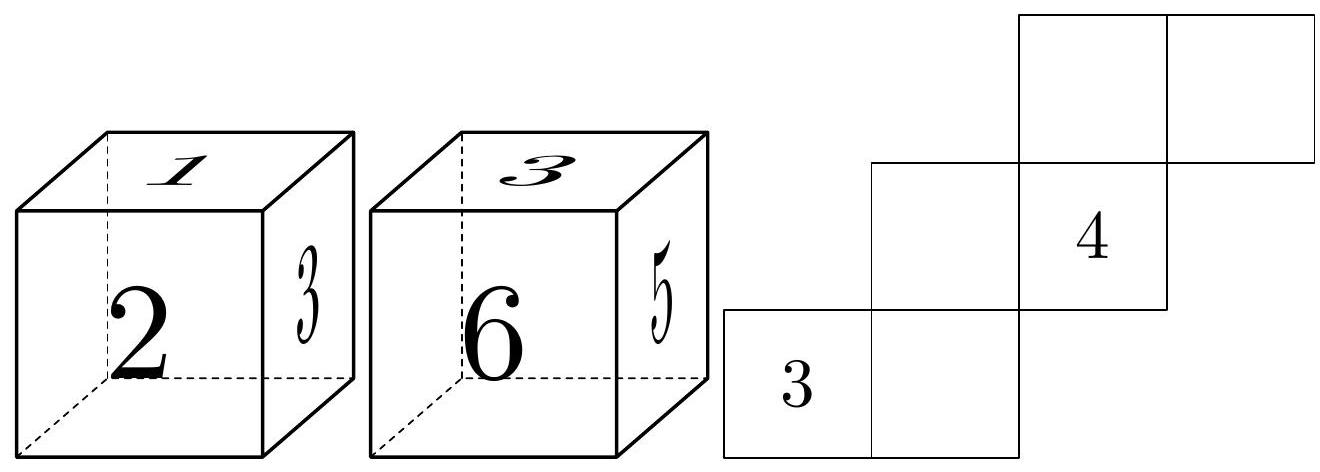
\includegraphics[max width=\textwidth, center]{2024_11_21_0a02dd0dee09c5119b68g-1}
  \item Jednakowym literom należy przyporządkować jednakowe cyfry, różnym różne. Wyznacz Ć, \(E, R, S, S, T, T, Y, Z\), aby działanie było poprawne.
\end{enumerate}

\[
\begin{array}{r}
T R Z Y \\
+T R Z Y \\
\hline \text { SZE'Ś }
\end{array}
\]


\end{document}